\documentclass[10pt,twocolumn,letterpaper]{article}

\usepackage{cvpr}
\usepackage{times}
\usepackage{epsfig}
\usepackage{graphicx}
\usepackage{amsmath}
\usepackage{amssymb}

\newenvironment{myitemize}
{ \begin{itemize}
    \setlength{\itemsep}{0pt}
    \setlength{\parskip}{0pt}
    \setlength{\parsep}{0pt}     }
{ \end{itemize}                  }

% Include other packages here, before hyperref.

% If you comment hyperref and then uncomment it, you should delete
% egpaper.aux before re-running latex.  (Or just hit 'q' on the first latex
% run, let it finish, and you should be clear).
\usepackage[breaklinks=true,bookmarks=false]{hyperref}

\usepackage{subcaption}

\cvprfinalcopy % *** Uncomment this line for the final submission

% \def\cvprPaperID{****} % *** Enter the CVPR Paper ID here
\def\httilde{\mbox{\tt\raisebox{-.5ex}{\symbol{126}}}}

% Pages are numbered in submission mode, and unnumbered in camera-ready
\ifcvprfinal\pagestyle{empty}\fi
% \setcounter{page}{1}

%%%%%%%%% DEFINE COMMANDS HERE %%%%%%%%% 

\newcommand{\norm}[1]{\lVert #1 \rVert}

\usepackage{todonotes}

\begin{document}

%%%%%%%%% TITLE
\title{Self-Supervised Feature Learning for Online Multi-Object Tracking}

\author{Bradley Collicott\\
Stanford University\\
{\tt\small collicott@stanford.edu}
\and
Mrunal Sarvaiya\\
Stanford University\\
{\tt\small mrunaljs@stanford.edu}
\and
Brian Weston\\
Stanford University\\
{\tt\small bweston@stanford.edu}
}

\maketitle

\thispagestyle{plain}
\pagestyle{plain}


\begin{abstract}
The multi-object tracking problem has a rich history in both model-based on data-driven approaches. This project serves as an investigation into improving the performance of an online multi-object tracking pipeline by introducing a self-supervised feature extraction network to provide dense feature representations of detected pedestrians in video. Multiple pretext tasks for self-supervised representation learning are explored and evaluated against a baseline method from literature on the downstream task of multi-object tracking. Results show that pre-trained networks can benefit from self-supervised fine-tuning, self-supervised learning is a viable replacement for feature learning, and a smaller network trained using metric learning for person re-identification can outperform larger fully-supervised networks. \footnote{Project code is available on \href{https://github.com/bcollico/cs231n_final_project}{GitHub}.}
\end{abstract}

\section{Introduction}
% This section introduces your problem, and the overall plan for approaching your problem.
Multi-object tracking (MOT) from video lies at the intersection of multiple core problems in computer vision. Described in \cite{Ciaparrone2020}, the MOT process consists of 4 stages: Detection, Feature Extraction, Motion Prediction, and Data Association. As explored in the seminal work by Fortmann, Bar-Shalom, and Scheffé in 1980 \cite{Fortmann1980}, there is a rich history of using the model-based methods of joint probabilistic data association (JPDA) and multi-hypothesis tracking (MHT) to solve MOT. Only recently have the advances in deep learning permeated the field with impressive results. DeepSORT \cite{Wojke2018}, one of the current state-of-the-art methods in real-time tracking, uses deep learning to provide a dense feature representation for use in a data association algorithm. In contrast, other works have attempted an end-to-end deep learning approach to MOT using modern architectures like recurrent neural networks and transformers \cite{Bastani2021, Meinhardt2021}. These methods prove effective but suffer high training time, computation, and memory costs.

The data association step (i.e. associating a detection with an existing trajectory) in MOT is widely considered to be the bottleneck for current performance. Therefore, this work seeks to investigate methods for improving feature representation to reduce the likelihood of ID switching (IDSW) and incorrect associations. Recent works have shown that self-supervised learning \cite{Jing2021} can imbue networks with the ability to learn context and salient features by solving a non-trivial pretext task at training time. The selection of pretext task depends on the downstream application, but in all cases the solution to the task is self-evident from the input, e.g. ordering a set of unordered video frames. With this in mind, the effectiveness of fine-tuning a pre-trained feature extraction network with multiple pretext tasks is investigated for improving MOT performance. Additionally, a fully self-supervised network is trained from scratch to compare learned features against that of a network trained in a fully-supervised manner.

\section{Related Work}

\subsection{Deep Learning in Multi-Object Tracking}
The roots of deep learning in MOT can be traced back to Wang et al. \cite{Wang2014Mot}, where deep features are learned for model-free tracking. The feature learning network resembles the modern autoencoder and includes pre-training to learn generic feature before transferring the model to multi-task learning on multiple objects. Since then, deep learning in multi-object tracking has exploded, largely due to advancements in object detection like as the Faster-RCNN \cite{FasterRCNN}. Although gains in deep MOT have largely been in detection and feature description, some works attempt deep affinity scoring to better match feature vectors \cite{DeepAffinity}, deep motion prediction with recurrent neural networks \cite{MotionPred}, and end-to-end solutions as alluded to with the rise of Transformers \cite{Meinhardt2021}.

\subsection{Self-Supervised Learning and Pretext Tasks}
Pretext tasks such as predicting image rotations are commonly used to train models to perform image classification on large datasets such as ImageNet. \cite{gidaris2018unsupervised} trains an AlexNet model to predict the correct image orientation in a self-supervised fashion. Similarly, \cite{PuzzleTask} introduces the jigsaw puzzle for self-supervised feature learning for transfer to classification and detection tasks. Towards using self-supervision for fine-tuning, Gidaris et al. \cite{Gidaris2019} demonstrated that few-shot learning could be improved by fine-tuning a pre-trained feature extraction network using self-supervised representation learning.

\section{Problem Approach and Methodology}
% Describe your problem precisely specifying the dataset to be used, expected results and evaluation.
The multi-object tracking problem can be decomposed into detection, feature extraction, motion prediction, and data association steps. To limit the scope of this project to self-supervised learning, the Deep SORT MOT pipeline \cite{Wojke2018} is adopted as the motion prediction and data association backend. Likewise, the public detections available with MOT datasets are used to allow for explicit comparison of the effectiveness between feature extraction networks rather than conflating with detector performance. All neural networks are implemented using PyTorch \cite{PyTorch}. The general multi-object tracking problem formulation, datasets, and methods of evaluation are discussed here.

\subsection{Multi-Object Tracking}
The objective of MOT is to detect the objects of interest and track them across multiple time steps. In the tracking-by-detection paradigm, this includes extracting the features of each detection and comparing with previously extracted features to associate each detection with the correct ID -- in this way, MOT is largely a data association problem. Further, online MOT addresses the problem of tracking objects in real-time by sequentially processing video frames.

\subsection{Pretext Tasks for Self-Supervised Fine-Tuning}
Pretext tasks are used in self-supervised learning to encourage neural networks to learn a representation that is useful for a separate downstream task. Given a image classification network pre-trained on a large dataset, the goal of this investigation is to augment the learned features using self-supervised training. For this task, a ResNet-18 \cite{Resnet} pretrained for classification on the ImageNet dataset \cite{imagenet_cvpr09} was selected as the backbone network. The ResNet architecture is shown in Fig. \ref{fig:resnet}.

\begin{figure}[h!]
    \centering
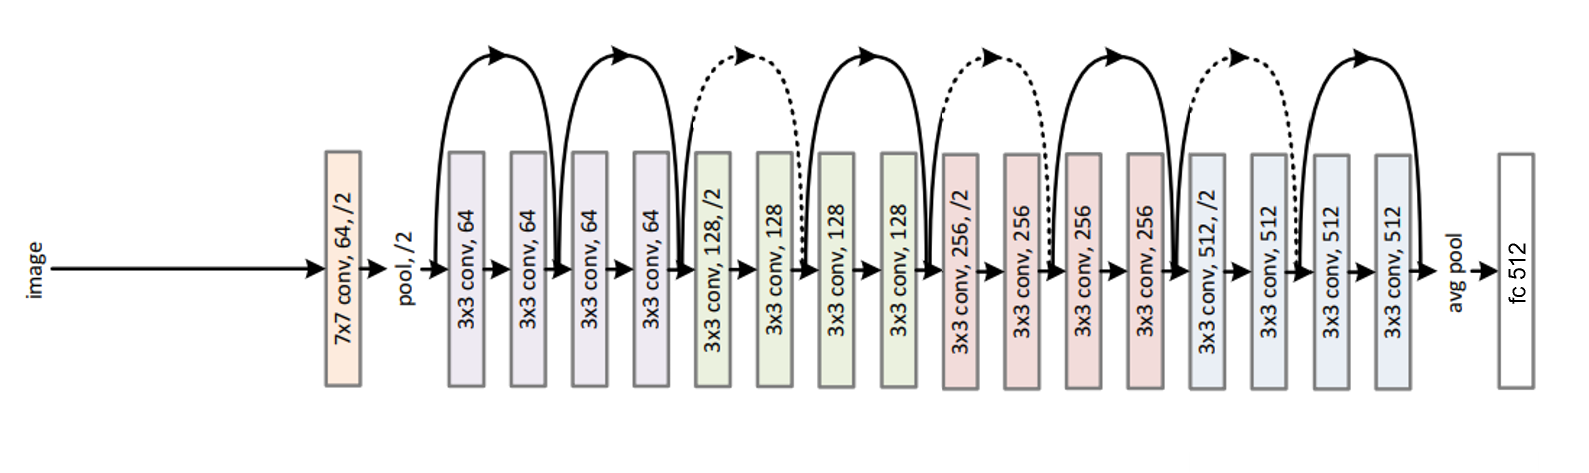
\includegraphics[width=\linewidth]{docs/reports/figs/resnet18.png}
    \caption{ResNet-18 Architecture (adapted from \cite{Resnet})}
    \label{fig:resnet}
\end{figure}

The ResNet-18 is an 18-layer network consisting of four 'residual blocks' that reduce the spatial extent of the image while increasing the number of dimensions. The network uses a global average pool before it's final fully-connected layer, resulting in a $512\times1\times1$ feature vector for use in the downstream application. This feature vector is the subject of interest for fine-tuning with self-supervised training -- two pretext tasks were selected to learn representations for evaluation on the downstream application of MOT.
\subsubsection{Puzzle Identification}
To encourage the pre-trained network to learn features relevant to that of a pedestrian, the puzzle identification task is considered. The traditional jigsaw puzzle task is such that the network is provided with 2 or more image segments, and the task to label each image segment with the correct ordering that would reconstruct the original image. In this case, the network is only presented with one image that is sampled as one of four quadrants from the original image. The target label is the number corresponding to the sampled quadrant. This scheme is visualized in Fig. \ref{fig:puzzle}.

The pre-trained ResNet-18 is used as the backbone architecture for this task. The network is augmented by removing the final fully-connected layer and re-initializing the weights in the final residual block using Xavier initialization \cite{XavierInit}. The global average pool is retained, and the output is flattened to a dimension of $512\times1$.

\subsubsection{Predicting Image Rotations}
One of the pretext tasks considered is predicting image rotations. The goal of this network is to learn features that enable it predict the correct 2D rotation that is applied to the image as an input. We start with the pretrained network used as the feature extractor in DeepSORT. We replace the last two layers (Batch and l2 normalization and Dense 10) with two fully connected layers as done in the original RotNet model \cite{Johnson20}. Finally, the loss function is the same as the one used in \cite{gidaris2018unsupervised} which is the negative log likelihood of the data set.


The model will be trained in a self supervised way using the cropped detection bound boxes from the MOT17 dataset. Since the model will learn to predict the correct rotations of humans, we expect the learned features to be useful in similar tasks, which in this case would be the affinity computation stage in the MOT tracking framework. 

\begin{figure}[h!]
    \centering
    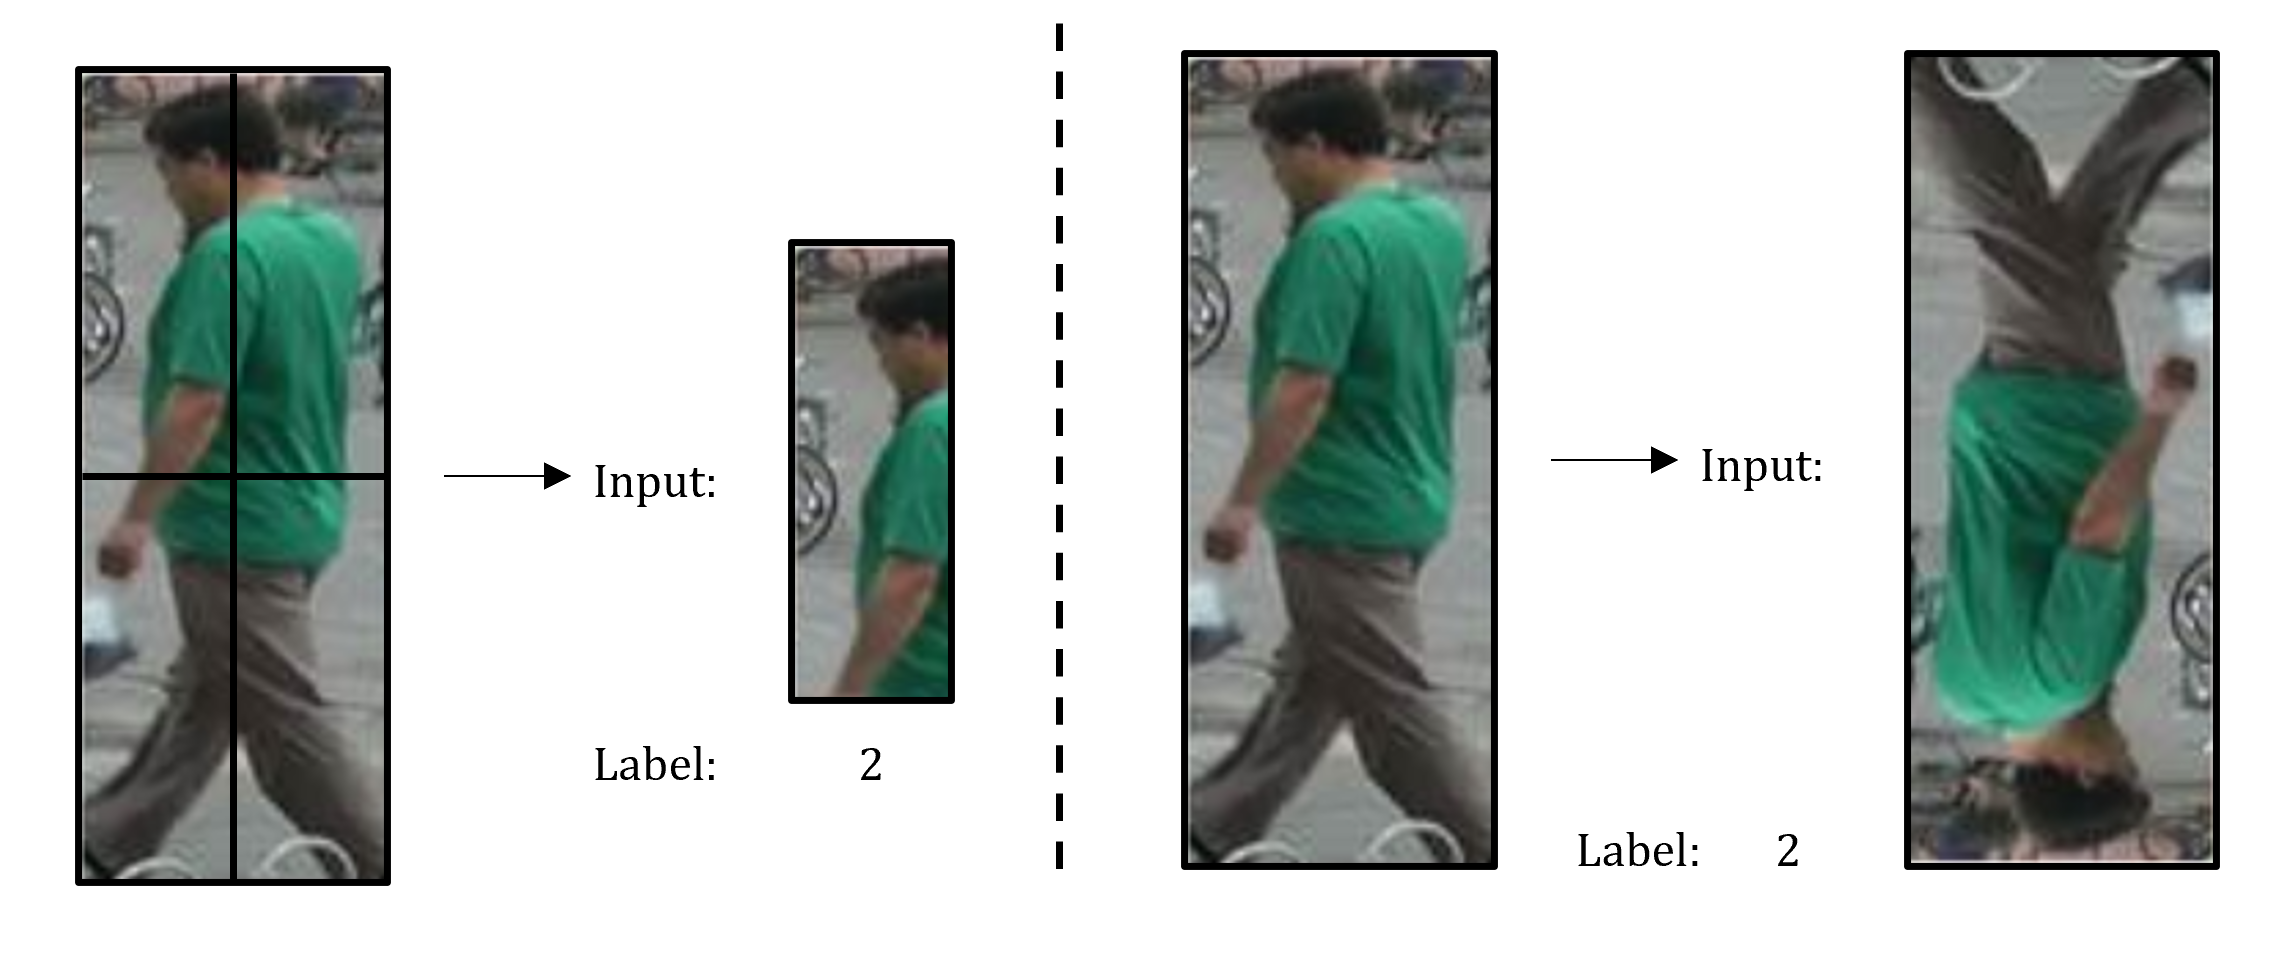
\includegraphics[width=0.95\linewidth]{docs/reports/figs/puzzle_task.png}
    \caption{Puzzle and Rotation Task Example}
    \label{fig:puzzle}
\end{figure}

\subsection{Fully Self-Supervised Learning}
\todo[inline]{Brian discuss reconstruction task for autoencoder.}
In contrast to using a pre-trained ResNet and fine-

An autoencoder is composed of an encoder and a decoder sub-models. The encoder compresses the input and the decoder attempts to recreate the input from the compressed version provided by the encoder. After training, the encoder model is saved and the decoder is discarded.

The encoder can then be used as a data preparation technique to perform feature extraction on raw data that can be used to train a different machine learning model.




% The final pretext task considered is colorization. The goal of the network is to learn embeddings to correctly predict the color in images from gray-scale version of the image. Starting again with the pretrained network as the inital feature extractor in DeepSORT, we strip the last two layers and the fine-tune new layers using this new self-supervised pretext task. 

% The model will be trained in a self-supervised way where we take the cropped detection bounding boxes from the MOT17 dataset. After the model is trained to learn color of the humans, clothes, and background, we expect the model to learn to track visual features and assist with data association problem \cite{Vondrick_2018_ECCV}.

\subsection{Baseline}
The baseline method will be a network trained using the deep cosine metric \cite{Wojke2018cosine} from the original DeepSORT feature extractor. This model was trained using a modified softmax loss to encourage features embeddings that are similar for input images of the same person and dissimilar to those for images of different people. The network used in DeepSORT is relatively shallow -- the architecture is shown in Fig. \ref{fig:baseline}. The network is substantially smaller than most modern CNN classifiers, and consideration will be given to the parameter count during discussion and comparisons.

\begin{figure}[h!]
    \centering
    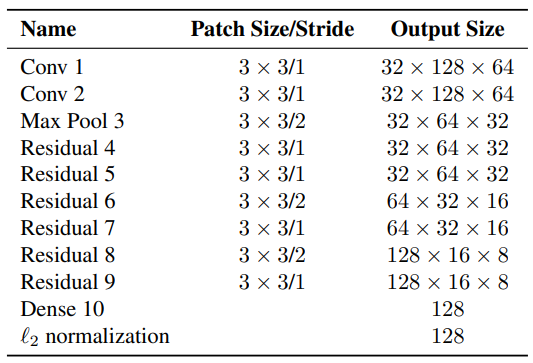
\includegraphics[width=0.9\linewidth]{docs/reports/figs/baseline_net.png}
    \caption{Baseline Network Architecture \cite{Wojke2018cosine}}
    \label{fig:baseline}
\end{figure}

\section{Datasets and Metrics}
Several datasets were used for training and the ultimate evaluation. Each dataset and accompanying evaluation metrics are briefly described here.
\subsection{MOT Evaluation}
The primary evaluation dataset will be the MOT17 \cite{MOT17} pedestrian tracking dataset. This dataset provides pedestrian detections from Faster-RCNN, Deformable Parts
Model (DPM), and scale-dependent pooling (SDP) object detectors with ground truth annotations for over 1300 unique IDs across over 11,000 frames. A sample frame from the MOT17 training data is shown in Figure 1.
\begin{figure}[h!]
    \centering
    \begin{subfigure}[b]{0.48\linewidth}
        \centering
        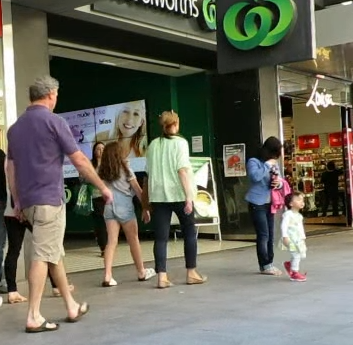
\includegraphics[width=\linewidth]{docs/reports/figs/MOT17_raw.png}
        \caption{Raw}
        \label{fig:my_label}
    \end{subfigure}
    \hfill
    \begin{subfigure}[b]{0.48\linewidth}
        \centering
        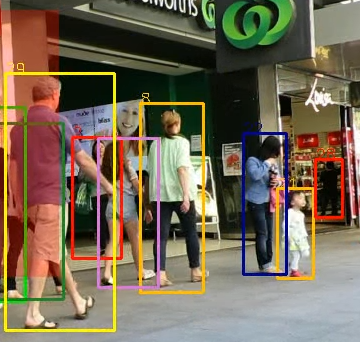
\includegraphics[width=\linewidth]{docs/reports/figs/MOT17_gt.png}
        \caption{Annotated}
        \label{fig:my_label}
    \end{subfigure}
    \caption{MOT17 Sample Scene}
\end{figure}
Ground truth annotations for the MOT17 dataset are not provided, so evaluation will be done with the training split. For this reason, additional datasets are used for the self-supervised fine-tuning and training.

\subsubsection{MOT Metrics}
The CLEAR MOT metrics established in \cite{Bernardin2008} will be used to evaluate tracking performance. We define the following terms for computing metrics:
\begin{myitemize}
    \item False Negative: Ground truth bounding box that cannot be associated with a hypothesis
    \item False Positive: Hypothesis that cannot be associated with a ground truth bounding box
    \item ID Switch: A change to a correct ground truth ID association
\end{myitemize}
The catch-all metric for tracking is the multi-object tracking accuracy (MOTA).
\begin{equation}
    MOTA = 1-\frac{FN+FP+IDSW}{GT}  \in (-\infty, 1]
\end{equation}
Where $FN$, $FP$, $IDSW$, and $GT$ are the number of false positives, false negatives, ID switches, and ground truth tracks across all frames, respectively. Another wholistic measure of MOT performance is the Multi-Object Tracking Precision (MOTP).
\begin{equation}
    MOTP = \frac{\sum_{t,i} IOU(d_i, \hat{d}_i)}{\sum{t} c_t}
\end{equation}
Where $IOU(d_i, \hat{d}_i)$ is the intersection-over-union of bounding box $i$ in frame $t$, and $c_t$ is the total number of ID matches in frame $t$.

In addition to the CLEAR MOT metrics, it is common to use the Mostly Tracked (MT) and Mostly Lost (ML) metrics to capture the number of trajectories correctly and incorrectly tracked for at least $80\%$ of the frames in which the tracks are present. Since this project will use public detections, the ML, MT, and IDSW metrics will be most informative for assessing performance.

\subsection{Self-Supervised Training Data}
The Motion Analysis and Re-Identification Set (MARS) \cite{zheng2016mars} served as the primary dataset for self-supervised fine-tuning on the rotation and puzzle pretext tasks. MARS contains bounding box images of over 1200 pedestrians from multiple camera views with the intent to train networks to recognize the same person from multiple views or across consecutive frames. A sample track from the MARS dataset is shown in \ref{fig:mars}.

\begin{figure}
    \centering
    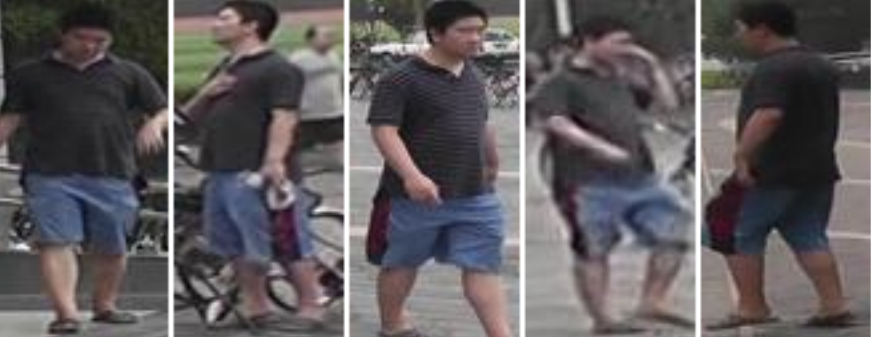
\includegraphics[width=0.95\linewidth]{docs/reports/figs/mars_example.png}
    \caption{MARS Dataset Sample Track}
    \label{fig:mars}
\end{figure}

The autoencoder network was trained on the Microsoft Common Objects in Context (MS COCO) dataset. \todo[inline]{Brian discuss your dataset and add a picture here.}

\subsubsection{Self-Supervised Training Metrics}
Puzzle prediction and rotation are both classification tasks which use the cross entropy (CE) loss. This can be computed for a batch of $N$ inputs with $C$ possible classes as:
\begin{equation}
    \mathcal{L}_{CE} = \sum_{i=1}^{N}\dfrac{e^{s_{y_i}}}{\sum_{j=1}^{C} e^{s_j}}
\end{equation}
where $s_i$ represents the output logit for class $i$.

The autoencoder is trained using self-supervised image reconstruction. This task uses a pixelwise $L_2$ loss between the input image $I$ and reconstructed image $\hat{I}$ for an image with height $H$ and width $W$.
\begin{equation}
    \mathcal{L}_{recon} = \sum_{i=1}^{N} \left(\sum_{u=1}^{H} \sum_{v=1}^{W} (I(u,v) - \hat{I}(u,v))^2\right)^{1/2}
\end{equation}
\todo[inline]{Brian please verify the autoencoder loss or correct this.}
\section{Results and Discussion}
\subsection{Pretext Task Training}
% Let's keep this brief so that we can spend more time on MOT and the resulting feature vectors. Potentially even cut this section out.
Although high performance on the pretext tasks is not the end-goal for this study, the training procedure and results for the self-supervised learning is briefly reviewed.
\subsubsection{Puzzle Task}
The puzzle task was trained using the Adam optimizer with a learning rate of $1$e$-5$ on mini-batches of size 128 for 10 epochs. The training data consisted of 25600 images from the MARS training split and was validated using a withheld set of 3200 images from the MARS test split. The network achieved a validation loss of $\mathcal{L}=0.824$ and validation accuracy of $92.2\%$. 
\subsubsection{Rotation Task}
The rotation task was trained using the Adam optimizer and cross entropy loss for 5 epochs. An initial grid search was run to find the initial set of values for the learning rate, betas, batch size and decay weight. After a finer search, the following values yielded the best results - learning rate: 6.7e-5, betas: (0.901, 0.986), batch size: 4, weight decay: 0.044. 
The training data consisted of 100000 images from the MARS dataset and was validated against a separate set of 100000 images. The network achieved a validation accuracy of $98.8\%$. 

\subsubsection{Image Reconstruction Task}

The autoencoder image reconstruction task was trained using an Adam optimizer with a learning rate of $1$e$-3$ on mini-batches of size 64 for 30 epochs. The training data consisted of 100,000 images from the 2017 unlabeled MS COCO dataset. The network achieved a validation loss of $\mathcal{L}=0.013$. As seen in Fig. \ref{fig:ae_reconstruction}, the autoencoder does quite well in reconstructing the original images with a noticeable blur due to the small bottleneck layer of size 512. 

\begin{figure}[h!]
    \centering
    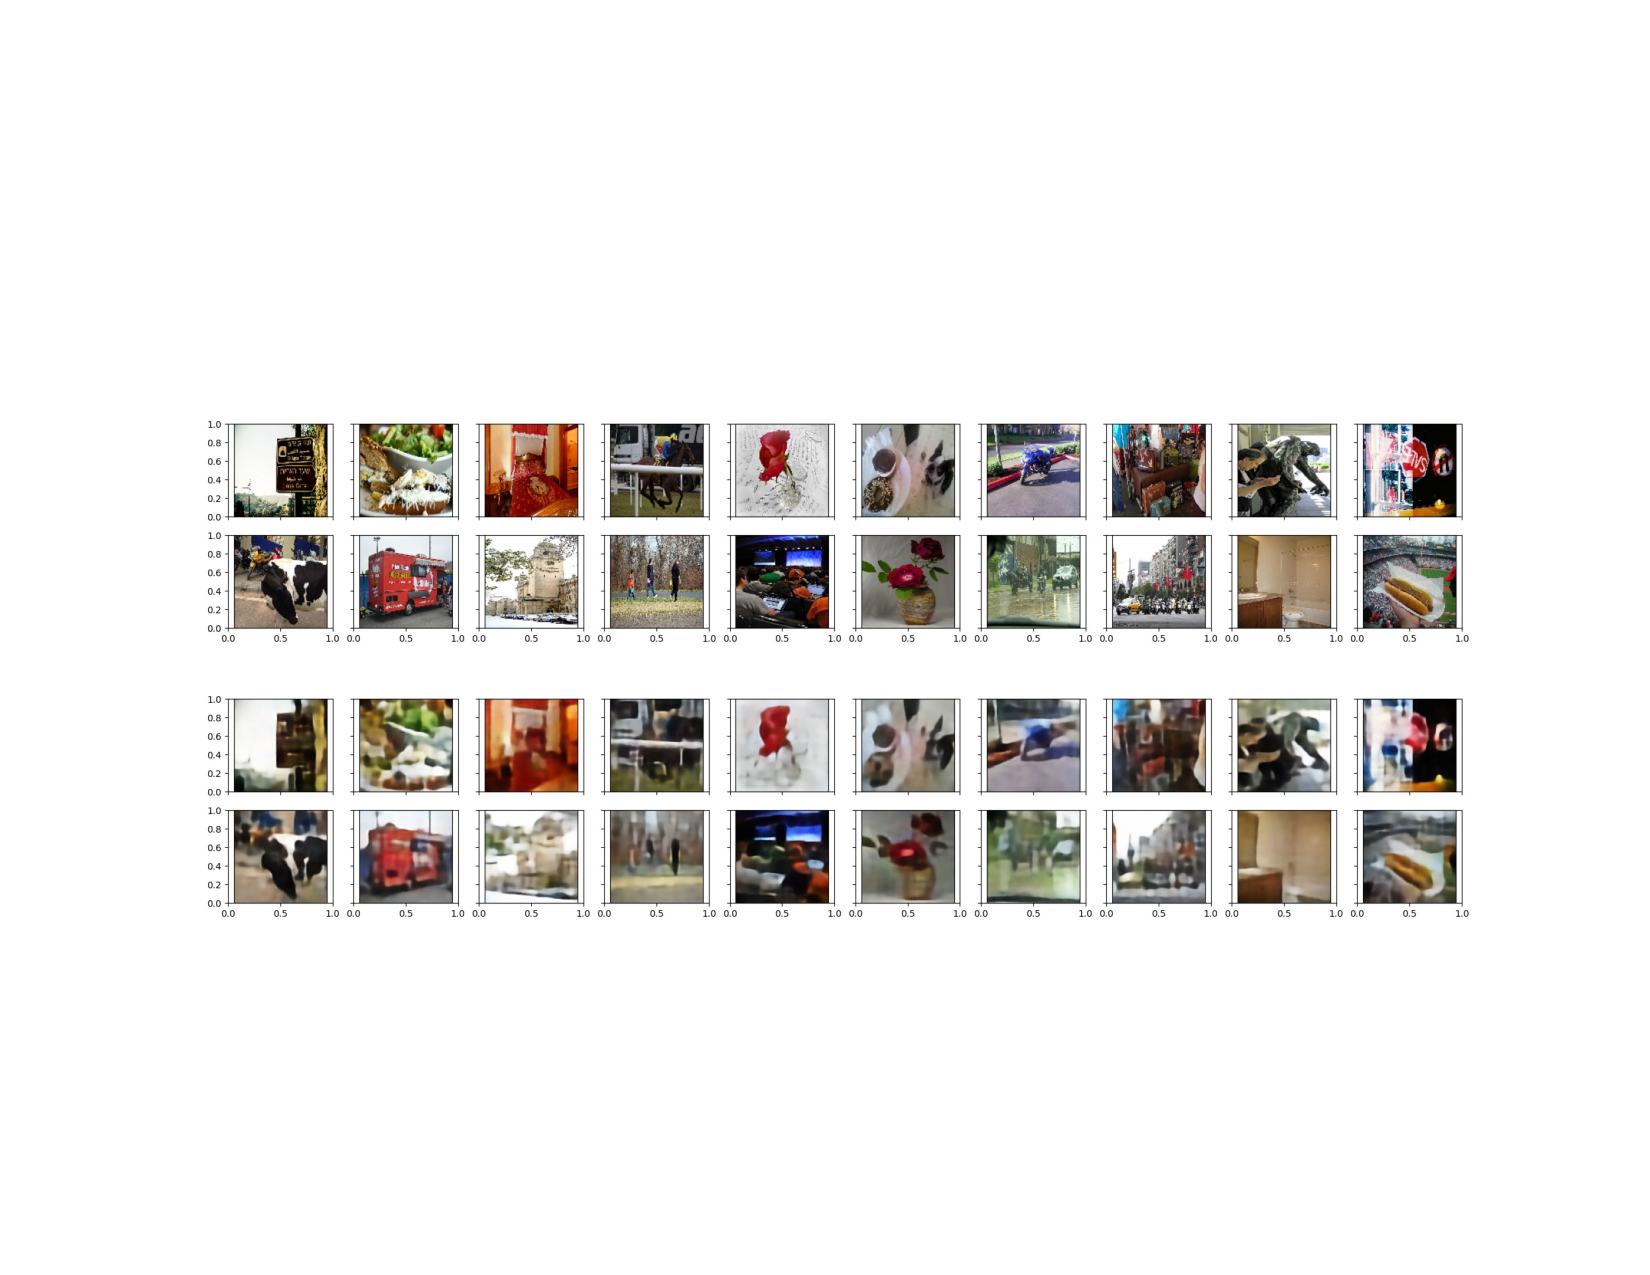
\includegraphics[width=1.\linewidth]{docs/reports/figs/reconstruction_original.pdf}
    \caption{Top figure: sample of 20 images from MS COCO dataset. Bottom figure: output reconstructed images from the trained autoencoder.}
    \label{fig:ae_reconstruction}
\end{figure}


\subsection{MOT Performance}
All networks were evaluated on the MOT17 dataset \cite{MOT17} using the same set of provided SDP, DPM, and FRCNN detections and the DeepSORT backend \cite{Wojke2018} for motion prediction and data association. Additionally, metrics were generated using TrackEval \cite{luiten2020IJCV}, the official evaluation tool for the MOT challenge. The 7 videos from the MOT17 training split were used for evaluation -- between the three detectors, these videos amount to 15948 frames and 1638 pedestrian tracks. Results for this evaluation are shown in Table \ref{tab:results}.

\begin{table*}[t!]
    \centering
    \begin{tabular}{|l|c|c|c|c|c|c|c|c|c|} 
         \hline & No. Params & MOTA $\uparrow$ & MOTP $\uparrow$ & MT $\uparrow$ & ML $\downarrow$ & IDSW $\downarrow$ & FRAG $\downarrow$ & FP $\downarrow$ & FN $\downarrow$  \\ \hline
         Baseline \cite{Wojke2018} & 2.8m & \textit{48.207} & \textit{83.746} & 340 & 573 & \textit{1458} & \textit{3680} & 161291 & \textit{11738}  \\ \hline \hline
         ResNet-18 \cite{Resnet} & 11.2m & 47.869 & \textbf{83.561} & 362 & 546 & 2176 & 4175& 159140& 14308 \\ \hline
         ResNet-18 + Puzzle  & 11.2m & 47.488 & 83.541 & 363 & \textbf{543} & 2412 & 4231 & 159183 & \textbf{14301} \\ \hline
         ResNet-18 + Rot. & 11.2m & 47.112&83.297 &354 &545 &4100 & 4603&159582 &14494 \\ \hline
         Autoencoder & 6.8m & \textbf{47.947} & 83.557&\textbf{367} &546 & \textbf{2064} & \textbf{4172} & \textbf{159054} &14243 \\ \hline
    \end{tabular}
    \caption{MOT17 Evaluation Results -- \textbf{Bold} = Best Results in this Study; \textit{Italics} = Baseline Obtains Best Results}
    \label{tab:results}
\end{table*}

As shown, baseline network generally outperforms the much larger pre-trained and fine-tuned networks, except in the Mostly Tracked, Mostly Lost, and False Positive metrics. The pre-trained does, however, provide competitive results without direct metric training or other feature augmentation for person re-identification.

Additionally, networks fine-tuned using self-supervised pretext tasks failed to outperform the baseline in most metrics, except for the MT, ML, and FP metrics as mentioned previously. These networks also generally do not exceed the performance of the pre-trained ResNet, despite achieving high accuracies in their respective pretext tasks. This indicates that the tasks may not have been difficult enough or contextually significant enough for the network to learn additional useful features, resulting in the weights of the re-trained layers adding little-to-no information to the feature vector and hampering the ResNet backbone. 

% speculation
The self-supervised autoencoder shows promising performance that rivals that of the ResNet-18 pre-trained in a fully-supervised manner on ImageNet. The autoencoder is also generally competitive with the baseline model with the exception of ID switching, which occurs approximately $41\%$ more often in the autoencoder than the baseline model. This suggests that self-supervised feature learning alone does not surpass metric learning for person re-identification, despite the upsides of full self-supervision.


\subsection{Feature tSNE}
% Mrunal add tSNE maps here and discuss how the original images compare to the reduced dimension features vectors in ResNet, Rotation, Autoencoder, etc.
To qualitatively analyze how effective the models are at differentiating different images of humans, we used tSNE to project the feature vectors generated on the MOT17 dataset onto a 2D plane. 

\begin{figure}[h!]
    \centering
    \begin{subfigure}[b]{0.5\linewidth}
        \centering
        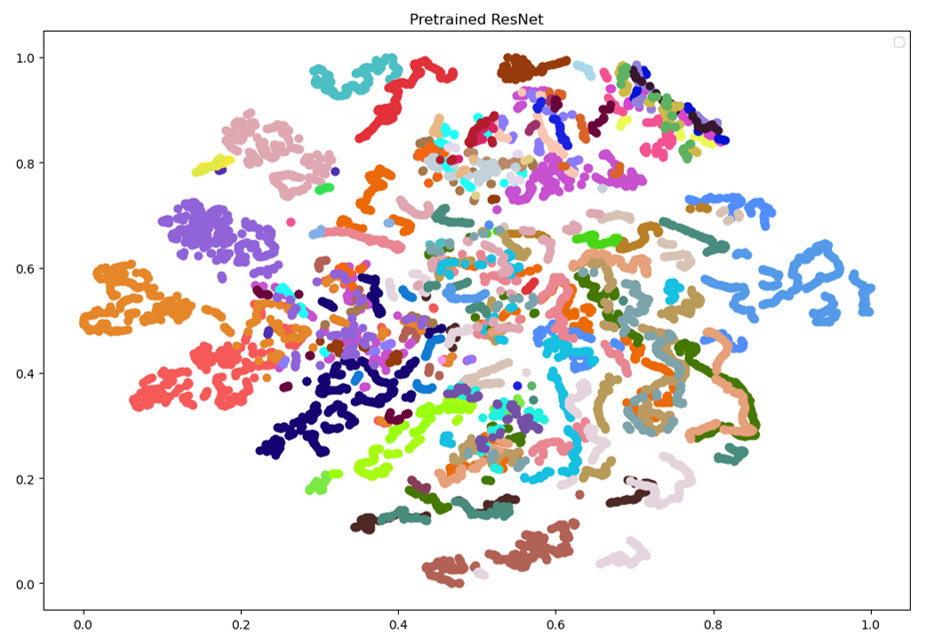
\includegraphics[width=\linewidth]{docs/reports/figs/tsne_resnet.png}
        \caption{tSNE: ResNet18}
        \label{fig:my_label}
    \end{subfigure}
    \hfill
    \begin{subfigure}[b]{0.47\linewidth}
        \centering
        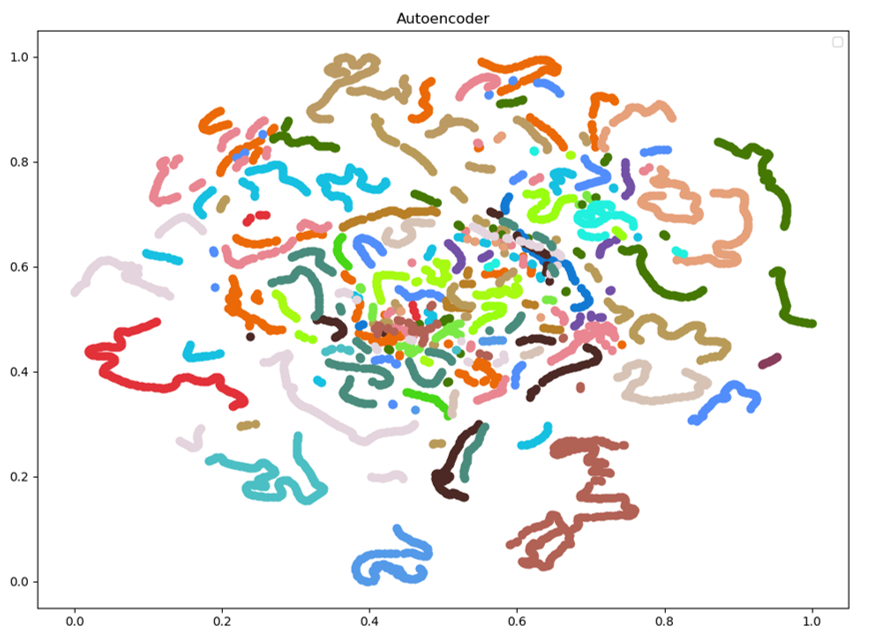
\includegraphics[width=\linewidth]{docs/reports/figs/tsne_auto_encoder.png}
        \caption{tSNE: Auto-Encoder}
        \label{fig:my_label}
    \end{subfigure}
    \caption{tSNE visualization}
\end{figure}

A pretrained ResNet-18 model generates distinct clusters for data points with the same labels and almost always only has only one cluster per label. The auto-encoder performs worse in this regard and has more than one cluster per label and often has multiple labels in the same vicinity. The auto-encoder, however, shows less overlap of clusters, leading to more distinct features between individuals. This qualitative analysis is supported by the quantitative results presented above. 

\subsection{Feature Vector Ablation}
% show curves for resnet or puzzle task feature vector length ablation and discuss
To investigate the sensitivity of the MOT process to feature vector length, the feature dimension was varied for the pre-trained ResNet-18 and the ResNet-18 fine-tuned on the puzzle task. The reduced dimension feature vectors were obtained from the ResNet using a 1D adaptive average pooling layer to reduce the dimensions from the original 512-dimension feature vector. The reduced dimension feature vector from the puzzle-task network was obtained by training networks with differing sizes of linear output layers, resulting in learned feature vectors of varying lengths. The effect of this variation is shown on in Fig. \ref{fig:featvec} for the MOTA and IDSW metrics.

\begin{figure}[h!]
    \centering
    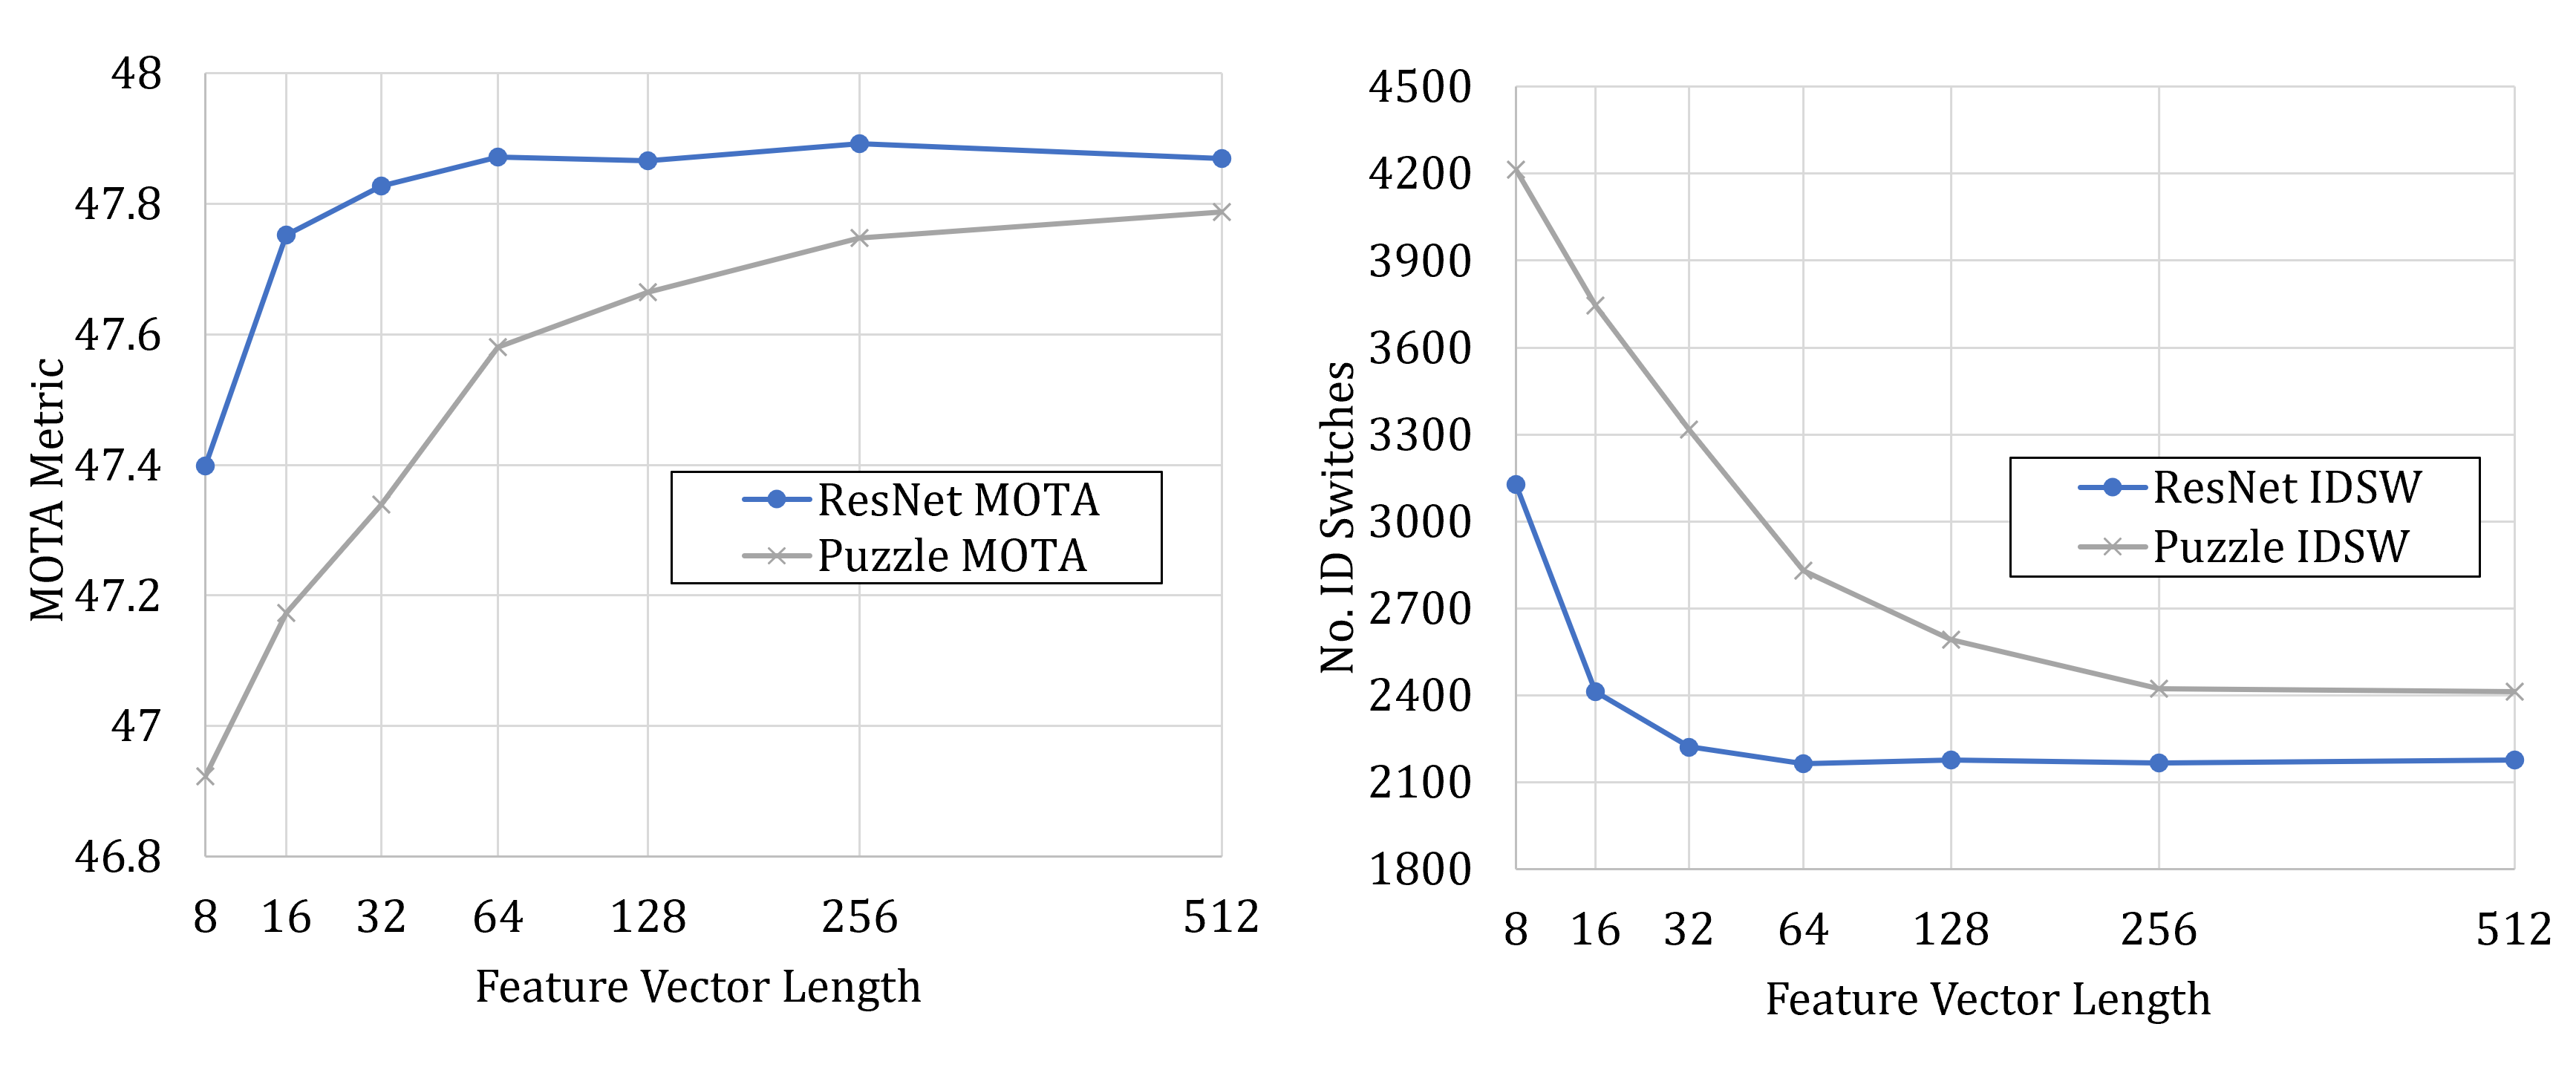
\includegraphics[width=\linewidth]{docs/reports/figs/feature_vec_effect.png}
    \caption{Effect of Varying Feature Vector Length on MOT Performance}
    \label{fig:featvec}
\end{figure}

As shown in the figure, the MOT performance of the pre-trained ResNet-18 is resilient to changes in feature vector length, whereas the puzzle-task network shows a pre-mature performance drop-off. This suggests that the feature vector produced by the puzzle network is comprised of less salient information than the ResNet, and that the self-supervised fine-tuning proved counterproductive.

With regard to comparing the performance of networks with different feature vector lengths, Fig. \ref{fig:featvec} suggests that the comparision is fair so long as the feature vector reaches a critical length in which the results no longer improve. For the ResNet-18, this is approximately 128 -- which is the dimension of the baseline feature extraction network. Since the performance of does not substantially increase for feature lengths greater than 128, fair comparison can be made between networks with feature vectors of different lengths.

\section{Conclusion}
Several methods were investigated for learning a feature embedding conducive for person re-identification via self-supervised learning. Two pretext tasks were used to fine-tune the learned feature embedding of a ResNet-18 pre-trained on ImageNet, and another network was trained from scratch using self-supervised image reconstruction. These methods were compared to a baseline metric learning method from literature on the MOT17 dataset. Although self-supervised learning is a burgeoning research area for learning useful feature embeddings from large sets of unlabelled data, it did not prove particularly effective in fine-tuning the learned features of the pre-trained network. The pre-trained ResNet-18 was shown to generally outperform or match the performance of the networks fine-tuned with pretext tasks. The self-supervised autoencoder performed similar to the pre-trained ResNet-18 with slight improvements in the MOTA, MT, IDSW, FRAG, and FP metrics. This suggests that fully self-supervised learning is a viable strategy for learning a useful feature embedding for person re-identification. 

Several additional observations were made regarding the requisite length of a feature embedding for person re-identification as well as a reduced-dimension analysis of the input and feature space for several networks. The feature vector length may be reduced to lessen memory and computational requirements at the loss of MOT performance beyond a certain threshold. It was also shown that the input space of the MOT17 dataset is able to be partitioned and clustered according to the ground truth pedestrian ID. The ResNet-18 pre-trained network and self-supervised autoencoder were also shown to produce feature embeddings that allow for clustering, further suggesting their suitability for person re-identification.

Although the self-supervised fine-tuning attempted in this effort was unsuccessful, there is future work in self-supervision for multi-object tracking. Extensions to this work could include: incorporating a meta-learning algorithm to guide the self-supervision process; training a self-supervised autoencoder jointly with metric learning tasks to improve performance on person re-identification; and merging the detection, feature description, and/or affinity calculation segments in a push towards end-to-end MOT.


\section{Contributions and Acknowledgements}
\todo[inline]{Brian and Mrunal add your contributions. Note that this section doesn't count towards our 6-page minimum}
This work makes use of several open-source repositories: \href{https://github.com/nwojke/deep_sort}{DeepSORT} for the MOT backbone and pre-trained baseline network; and \href{https://github.com/JonathonLuiten/TrackEval}{TrackEval} for evaluating the MOT metrics.

Group member contributions are as follows: B.C. led report writing and contributed the core PyTorch code framework, puzzle pretext task, model evaluations, and feature vector ablation study. M.S. .... B.W. ....



{\small
\bibliographystyle{ieee}
\bibliography{references}
}

\end{document}

